\documentclass[12pt, a4paper]{article}
\usepackage[UKenglish]{babel}
\usepackage[utf8]{inputenc}
\usepackage{mathtools} % an extension of amsmath
\usepackage{amsthm, amssymb, amsfonts, amstext}
\usepackage{longtable}
\usepackage{tocloft}
\usepackage{geometry}
\usepackage{algpseudocode}
\usepackage{multicol}
\geometry{margin=27mm}
\usepackage{listings}
\usepackage{xcolor,colortbl}
\usepackage{wrapfig}
\usepackage{graphicx}
\usepackage{array}
\usepackage{tabularx}
\usepackage{makecell}
\usepackage{tcolorbox}
\usepackage{enumitem}
\renewcommand\theadalign{bc} % to leave lines inside a table
\renewcommand\theadgape{\Gape[4pt]}
\renewcommand\cellgape{\Gape[4pt]}
\definecolor{codegreen}{rgb}{0,0.6,0}
\definecolor{codegray}{rgb}{0.5,0.5,0.5}
\definecolor{codepurple}{rgb}{0.58,0,0.82}
\definecolor{backcolour}{rgb}{0,0,0}
\definecolor{pageBG}{rgb}{0,0,0}
\usepackage{hyperref}
\hypersetup{
    colorlinks=true,
    linkcolor=blue,
    filecolor=magenta,
    urlcolor=cyan,
}
\lstdefinestyle{mystyle}{
    backgroundcolor=\color{white},
    commentstyle=\color{cyan},
    keywordstyle=\color{red},
    numberstyle=\tiny\color{red},
    stringstyle=\color{codepurple},
    basicstyle=\ttfamily\footnotesize\color{codegreen},
    breakatwhitespace=false,
    breaklines=true,
    captionpos=b,
    keepspaces=true,
    numbers=left,
    numbersep=5pt,
    showspaces=false,
    showstringspaces=false,
    showtabs=false,
    tabsize=4
}
\lstset{style=mystyle}
\urlstyle{same}
\usepackage{cleveref}

\newtheorem{theorem}{Theorem}[section]
\theoremstyle{definition}
\newtheorem{definition}{Definition}[section]
\newtheorem*{claim}{Claim}
\theoremstyle{remark}
\newtheorem*{remark}{Remark}
% \numberwithin{equation}{section}
\newcommand{\textsb}{\textsubscript}

\title{Algorithms Analysis \& Design\\Dynamic Programming}
\author{Aditya Harikrish\\2020111009}
\date{}

\begin{document}
\maketitle
\tableofcontents
\newpage

\section{Introduction}
Dynamic programming is a technique to solve computational problems by breaking them down into smaller and simpler subproblems. Problems that can be broken down in this manner are said to have the `optimal substructure property'.

In general, we can split dynamic programming problems into three steps, of which the first two need not be followed in any particular order. They are as follows.
\begin{enumerate}
    \item The base case. These are some of the already known cases whose answers are known beforehand. Base cases are useful for stopping recursive call stacks and providing some information that allows us to base other solutions off of.
    \item The transition function. This is the function which translates a problem into a set smaller subproblems.
    \item The final answer. We need to extract the final answer from all the computation that has been performed.
\end{enumerate}

\subsection{Example}
\begin{tcolorbox}
    \textbf{The Problem:} Given a natural number $n$, find the number of different ways to write it as a sum of 1, 3, and 5.
\end{tcolorbox}
For example, for $n = 6$, the answer is 7.
\begin{equation*}
    \begin{split}
        6 &= 1+1+1+1+1+1 \\
        &= 1+1+1+3\\
        &= 1+1+3+1\\
        &= 1+3+1+1\\
        &= 3+1+1+1\\
        &=1+5\\
        &= 5+1
    \end{split}
\end{equation*}

Before defining the problem as a set of subproblems, let us define $S_n$ to be the number of ways to write $n$ as a sum of 1, 3, and 5.

Let $n = a_1 + \ldots a_m$ be a solution. Notice that if $a_m = 5$, then $a_1 + \ldots a_{m-1} = n - 5$. Therefore, there are $S_{n-5}$ solutions that end in $a_m = 5$.

The sum can only end in three 1, 3, and 5. Therefore,
\begin{equation}
    S_n = S_{n-1} + S_{n-3} + S_{n-5}.
\end{equation}

The recurrence must end in some base cases. Here,
\begin{itemize}
    \item $S_0 = 1$
    \item $S_i = 0$ for $i < 0$
\end{itemize}

The pseudocode is given below.
\begin{lstlisting}
function S(n):
    if n < 0: return 0
    if n = 0: return 1
    return S(n-1) + S(n-3) + S(n-5)
\end{lstlisting}

\section{Fibonacci Sequence}
One of the most popular sequences, the Fibonacci sequence is defined as follows.
\begin{enumerate}
    \item The first element is 0 and the second element is 1.
    \item Each subsequent element is the sum of the previous two elements.
\end{enumerate}

$F_i$ denotes the $i$th Fibonacci number. From the definition,
\begin{equation}
    F_i = \begin{cases}
        0                 & \text{ if } i = 0 \\
        1                 & \text{ if } i = 1 \\
        F_{i-1} + F_{i-2} & \text{ if } i > 1
    \end{cases}
\end{equation}

\begin{tcolorbox}
    \textbf{The Problem:} Given a positive integer $n$, find the Fibonacci sequence from $F_0$ to $F_n$, i.e. the first $n+1$ elements.
\end{tcolorbox}

\subsection{Without Memoisation: The Naive Solution}
The simplest solution is to directly implement the definition using recursion, shown below.
\begin{lstlisting}[language=C++]
uint64_t Without_Memoisation(std::vector<uint64_t>& FibArray, uint64_t n) {
    if (n <= 1)
        FibArray[n] = n;
    else
        FibArray[n] = Without_Memoisation(FibArray, n - 1) + Without_Memoisation(FibArray, n - 2);
    return FibArray[n];
}
\end{lstlisting}
% 
However, this solution has a serious drawback - it runs in exponential time. For all $\text{fib}(i)$ where $i \geq 2$, two functions are called - $\text{fib}(i-1)$ and $\text{fib}(i-2)$. And each of these called functions call two more unless they're the first two elements in the sequence. This generates a binary tree of recursive calls, with almost $2^n$ recursive calls.

\begin{figure}[!h]
    \centering
    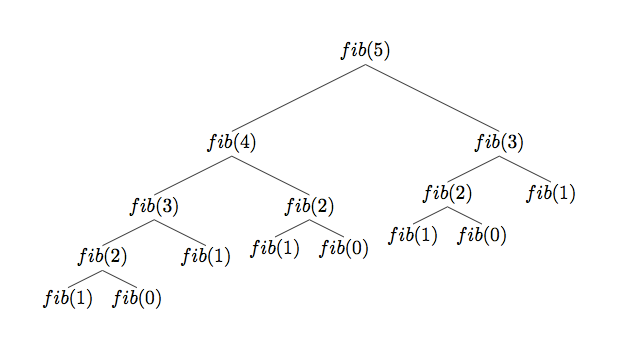
\includegraphics[scale=0.9]{img/Fibonacci - Call Tree.png}
    \label{fig:fib_calltree}
    \caption{The call tree for $\text{fib}(5)$ (without memoisation)}
\end{figure}

Refer to Figure \ref{fig:fib_calltree} for an example.

\subsection{With Memoisation}
Memoisation is a neat little trick that is widely used to speed up algorithms. Simply put, memoisation is the technique of storing computed results so that the computation need not take place again to determine the same result.

For the Fibonacci sequence, let us create an array called `FibArray' where
\begin{equation*}
    \text{FibArray}[i] = F_i.
\end{equation*}

When computing the first $n+1$ elements, initially, FibArray is empty. Whenever the function computes the $i$th Fibonacci number, it stores the value in $\text{FibArray}[i]$. Following this, whenever another function needs the value of $F_i$, the value is returned from $\text{FibArray}[i]$ in $O(1)$, which is a huge improvement the earlier exponential time complexity.

Here, each function call from $\text{fib}(0)$ to $\text{fib}(n)$ computes the value of its corresponding Fibonacci number only once. Thus, all but one instance of each of these function calls occur in $O(1)$. The time complexity is $O(n)$. Refer to Figure \ref{fig:fibograph} for a comparison in the performace of the two solutions to the Fibonacci Sequence problem.

\begin{lstlisting}[language=C++]
std::vector<uint64_t> FibArray(n + 1, 4);
uint64_t With_Memoisation(std::vector<uint64_t>& FibArray, uint64_t n) {
    // The default value to fill the array is 4, because 4 is not a Fibonacci number
    // Checking if the value is present in the memo
    if (FibArray[n] != 4) return FibArray[n];

    // Value not present in memo at this point
    if (n <= 1)
        FibArray[n] = n;
    else
        FibArray[n] = With_Memoisation(FibArray, n - 1) + With_Memoisation(FibArray, n - 2);
    return FibArray[n];
}
\end{lstlisting}

\begin{figure}[!h]
    \centering
    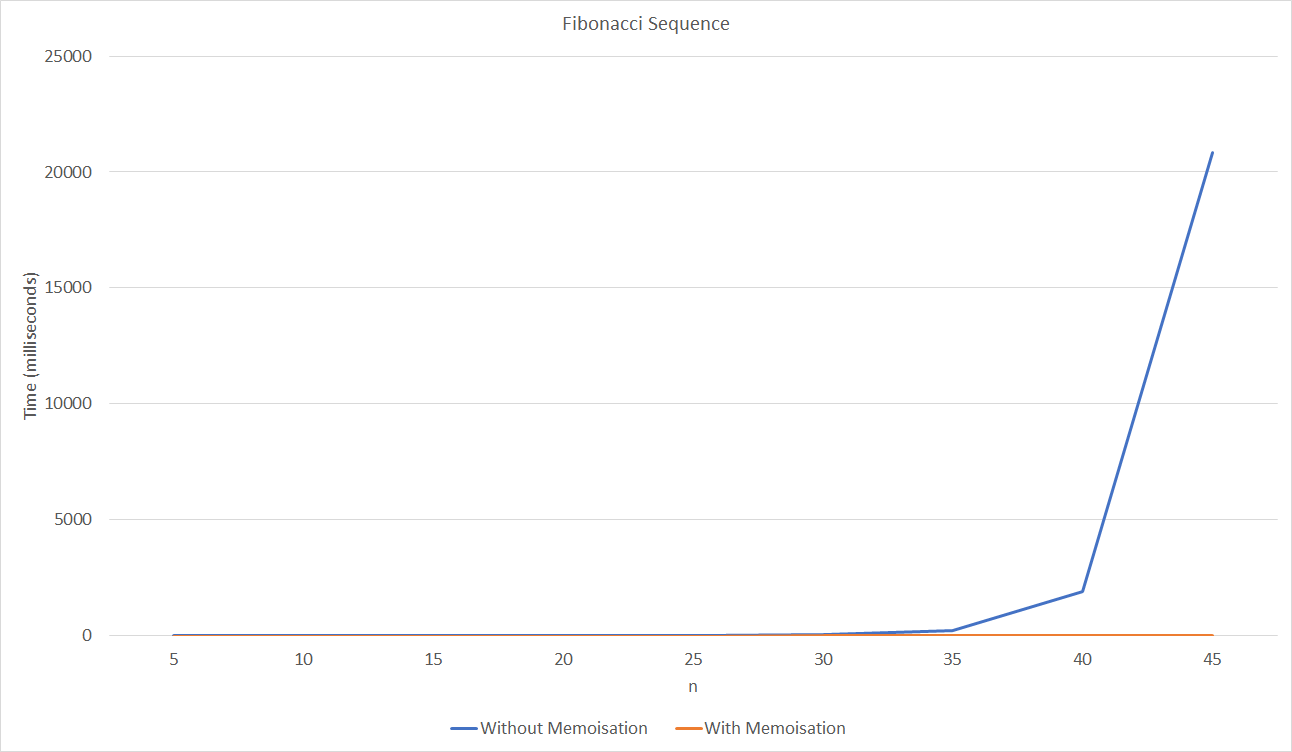
\includegraphics[scale=0.45]{img/Fibonacci - Memo vs No Memo Graph.png}
    \label{fig:fibograph}
    \caption{Time taken to calculate the first $n+1$ elements of the Fibonacci sequence with and without memoisation}
\end{figure}

\section{Frog Jump}
\begin{tcolorbox}
    \textbf{The Problem:} There are $n$ stones in a line (numbered $0, 1,\ldots,n-1$) and a frog is on Stone 0. Each stone has a height. The $i$th stone has height $h_i$. The cost of jumping from Stone $i$ to Stone $j$ is $|h_j - h_i|$. Find the minimum cost for the frog to go from Stone 0 to Stone $n-1$.
\end{tcolorbox}

\subsection{2 Steps} \label{sec:frog2steps}
In this version of the problem, if the frog is on Stone $i$, it can only jump to Stone $i+1$ or Stone $i+2$ in a single jump.

Let us create an array called `dp' such that
\begin{equation} \label{eq:frogjumpdp}
    \text{dp}[i] = \text{minimum cost for the frog to go from Stone $0$ to Stone $i-1$}.
\end{equation}

\begin{description}
    \item[Transition function.] We notice that the $i$th stone can be reached from either the $(i-1)$th stone or the $(i-2)$th stone (for $i \geq 2$). That means that dp[$i$] is the minimum of these two cases.
        \begin{equation}
            \text{dp}[i] = \min\{\text{dp}[i-1] + |h_i - h_{i-1}|, \text{dp}[i-2] + |h_i - h_{i-2}|\} \text{ when } i \geq 2
        \end{equation}
    \item[Base cases.] There are at most two stones which do not have two preceding stones - Stone 0 and Stone 1. Thus, we shall manually define dp[0] and dp[1] beforehand.
        \begin{gather}
            \text{dp}[0] = 0 \text{ as the frog starts at Stone 0, and} \\
            \text{dp}[1] = |h_1 - h_0|.
        \end{gather}
    \item[Final answer.] From \cref{eq:frogjumpdp}, our final answer is dp[$n-1$].
\end{description}
\begin{lstlisting}[language=C++]
#include <iostream>
#include <vector>
int main(void) {
    int n;
    std::cin >> n;
    std::vector<int> h(n), dp(std::max(n, 2));
    for (auto &it : h) std::cin >> it;

    dp[0] = 0;
    dp[1] = abs(h[1] - h[0]);

    for (int i = 2; i < n; ++i) {
        dp[i] = std::min(dp[i - 1] + abs(h[i] - h[i - 1]),
                        dp[i - 2] + abs(h[i] - h[i - 2]));
    }

    std::cout << dp[n - 1] << "\n";

    return 0;
}
\end{lstlisting}

\subsection{K Steps}
In this version of the problem, if the frog is on Stone $i$, it has $k$ different stones which it can jump to in one go: Stones $i+1$, $i+2,\ldots$ ,$i+k$.
The solution is just an extension and a generalisation of \cref{sec:frog2steps}.
We use the same definition for the dp array as shown in \cref{eq:frogjumpdp}.

\begin{description}
    \item[Transition function.] The $i$th stone can be reached directly from any one of Stones $i-1$, $i-2, \ldots,$ $i-k$ (for $i \geq k$). That means that dp[$i$] is the minimum of these $k$ cases.
        \begin{equation}
            \text{dp}[i] = \min_{j = 1,2,\ldots,n}\{\text{dp}[i-j] + |h_i - h_{i-j}|\} \text{ when } i \geq k
        \end{equation}
    \item[Base cases.] There are at most $k$ stones which do not have $k$ preceding stones - Stones 0 through $k-1$. Thus, we shall manually define dp[0], dp[1],...,dp[$k-1$] beforehand.
        \begin{gather}
            \text{dp}[0] = 0 \text{ as the frog starts at Stone 0, and} \\
            \text{dp}[i] = \min_{j = 0, 1, \ldots, i-1} \{ dp[j] + |h_i - h_j| \} \text{ when } i < k.
        \end{gather}
    \item[Final answer.] From \cref{eq:frogjumpdp}, our final answer is dp[$n-1$].
\end{description}

\begin{lstlisting}[language=C++]
int MinCostDP(const std::vector<int>& h, int k) {
    int n = h.size();
    std::vector<int> dp(n);
    dp[0] = 0;

    for (int i = 1; i < n; ++i) {
        int curr_min = dp[i - 1] + abs(h[i] - h[i - 1]);

        for (int j = i - 2; j >= i - k && j >= 0; --j) {
            curr_min = std::min(curr_min, dp[j] + abs(h[i] - h[j]));
        }

        dp[i] = curr_min;
    }

    return dp[n - 1];
}
\end{lstlisting}

\section{Longest Increasing Subsequence (LIS)}
A subsequence $L$ of a sequence $S$ is a sequence that can be obtained by deleting some or none of the elements in $S$, without changing the order in which the elements appear.
\begin{tcolorbox}
    \textbf{The Problem:} Given a sequence of $n$ numbers, $a_0, a_1,\ldots,a_{n-1}$, find the longest subsequence of this sequence that is strictly increasing. If there are multiple such subsequences, find any of them.
\end{tcolorbox}
The brute-force approach would be to check every possible subsequence, but that would take exponential time as there are $2^n$ possible subsequences in a sequence of $n$ elements. Thus, we shall not discuss this approach.

\subsection{Version 1 - $O(n^2)$}
Let us define an array called `dp' as follows.
\begin{equation}
    \text{dp}[i] = \text{length of the LIS ending with } a_i.
\end{equation}
Let us also define an array called `prev' such that prev[$i$] is the index of the element (in the sequence $a_0,\ldots,a_{n-1}$) immediately preceding $a_i$ in the longest increasing subsequence that $a_i$ is a part of.
\begin{description}
    \item[Base cases.] We observe that dp$[i]$ must be at least one as the subsequence that contains only $a_i$ is also increasing. So, we initialise dp$[i] = 1$ and prev$[i] = -1$ (since we have no information about any LIS in the beginning) for all $i = 0, 1,\ldots, n-1$.
    \item[Transition Function.] Observe that for some $j < i$, if
        \begin{enumerate}
            \item $a_i > a_j$ (i.e., it is possible for $a_i$ to succeed $a_j$ in an increasing subsequence), and
            \item dp$[i]$ < dp$[j] + 1$,
        \end{enumerate}
        then we set
        \begin{itemize}
            \item $\text{dp}[i] = \text{dp}[j] + 1$, and
            \item $\text{prev}[i] = j$
        \end{itemize}
        We also keep track of the last index of the longest increasing subsequence known so far (in the variable `last\_index\_of\_LIS') along with its length (in the variable `max\_length').
    \item[Final answer.] The length of the LIS is `max\_length'. To find the LIS itself, start from $i$ = last\_index\_of\_LIS and go to prev[$i$] and update $i$ to prev$[i]$ until prev$[i]$ is -1. Note that this gives the LIS in reverse order, so you might prefer to reverse this list.
\end{description}
\begin{lstlisting}[language=C++]
int LIS::lengthOfLIS_v1(const std::vector<int>& a) {
    if (a.size() < 1) return 0;
    std::vector<int> dp(a.size(), 1);    /* DP[i] = length of the LIS ending with a[i] */
    std::vector<int> prev(a.size(), -1); /* Only needed to find the LIS itself in addition to its length */
    int max_length = 1;
    int last_index_of_LIS = -1;
    for (int i = 1; i < a.size(); ++i) {
        for (int j = 0; j < i; ++j) {
            if (a[i] > a[j] && dp[j] + 1 > dp[i]) {
                dp[i] = dp[j] + 1;
                prev[i] = j;
            }
        }
        if (dp[i] > max_length) {
            max_length = dp[i];
            last_index_of_LIS = i;
        }
    }

    /* Print the LIS */
    std::vector<int> LIS_in_reverse;
    for (auto i = last_index_of_LIS; i >= 0;) {
        LIS_in_reverse.push_back(a[i]);
        i = prev[i];
    }
    std::cout << "LIS: ";
    for (auto it = LIS_in_reverse.rbegin(); it != LIS_in_reverse.rend(); ++it) {
        std::cout << *it << " ";
    }
    std::cout << "\n";
    return max_length;  // Length of the LIS
}
\end{lstlisting}

\subsubsection{Time Complexity}
We iterate through each element in the array a. For each element, we go through each of the previous elements, in $O(1)$ for each of the previous elements. Thus, the overall time complexity is $O(n^2)$.

\subsection{Version 2 - $O(n \log n)$}
Let use create an array called `$s$' defined as follows.
\begin{equation}
    s[i] = \text{ index of the smallest integer that ends an increasing sequence of length } i.
\end{equation}
% 
We define an array called `$parent$' such that $parent[i]$ is the index of the previous element in the LIS containing $a_i$.
Now, iterate through the sequence. Let the index of the current iteration be $i$.

\begin{enumerate}
    \item If $a_i$ is greater than the last element in $s$, then this means that we have found a larger increasing sequence than the one currently known and thus, we append $a_i$ to $s$.
    \item Otherwise, we find the smallest element in whose index is in $s$ which is greater than or equal to $a_i$ and change it to $a_i$. Notice that this element can be found using binary search in $O(n \log n)$ because $s$ is always sorted.
\end{enumerate}
The length of the LIS is simply the length of $s$. To find the LIS itself, we update the $parent$ array as follows:
\begin{enumerate}
    \item If $a_i$ is greater than the last element in $s$, then $parent[i] = \text{the last element in } s$ since the parent of the new element is the previously last element.
    \item Otherwise, using the the index of the smallest element found using binary search earlier, (say `$index$'), we set $parent[i] = s[index - 1]$.
\end{enumerate}

\begin{lstlisting}[language=C++]
int LIS::lengthOfLIS_v2(const std::vector<int>& a) {
    if (a.size() < 1) return 0;
    std::vector<int> s; /* s[i] = index of the smallest integer that ends an increasing sequence of length i */
    s.push_back(0);
    std::vector<int> parent(a.size(), -1);
    for (int i = 1; i < a.size(); ++i) {
        if (a[i] > a[s.back()]) {
            parent[i] = s.back();
            s.push_back(i);
        } else {
            /* Binary search in s for the smallest integer >= a[i] */
            int l = 0, r = s.size() - 1;
            int mid = l + (r - l) / 2;
            int index = r; /* Index of the target in s */
            while (l <= r) {
                mid = l + (r - l) / 2;
                if (a[s[mid]] >= a[i]) {
                    index = std::min(index, mid);
                    r = mid - 1;
                } else {
                    l = mid + 1;
                }
            }
            if (index - 1 >= 0)
                parent[i] = s[index - 1];
            else
                parent[i] = -1;
            s[index] = i;
        }
    }

    /* Print the LIS */
    std::vector<int> LIS_in_reverse;
    for (int i = s.back(); i >= 0;) {
        LIS_in_reverse.push_back(a[i]);
        i = parent[i];
    }
    std::cout << "LIS: ";
    for (auto it = LIS_in_reverse.rbegin(); it != LIS_in_reverse.rend(); ++it) {
        std::cout << *it << " ";
    }
    std::cout << "\n";

    return s.size();  // Length of the LIS
}
\end{lstlisting}

\subsubsection{Time complexity}
We iterate through each of the $n$ elements in the sequence, and perform one binary search that takes $O(\log n)$ time. Thus, the overall time complexity is $O(n \log n)$.

\begin{figure}[!h]
    \centering
    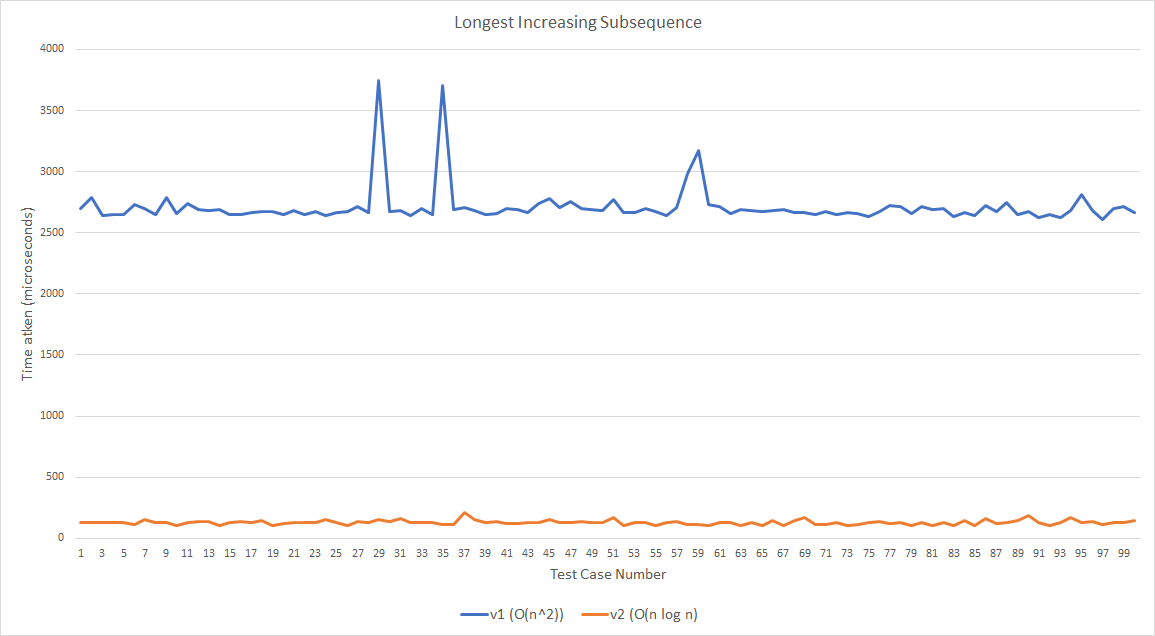
\includegraphics[scale=0.5]{img/LIS - constant n (1000).png}
    \label{fig:LIS1}
    \caption{LIS: time taken for $n = 1000$ over 100 test cases}
\end{figure}
\begin{figure}[!h]
    \centering
    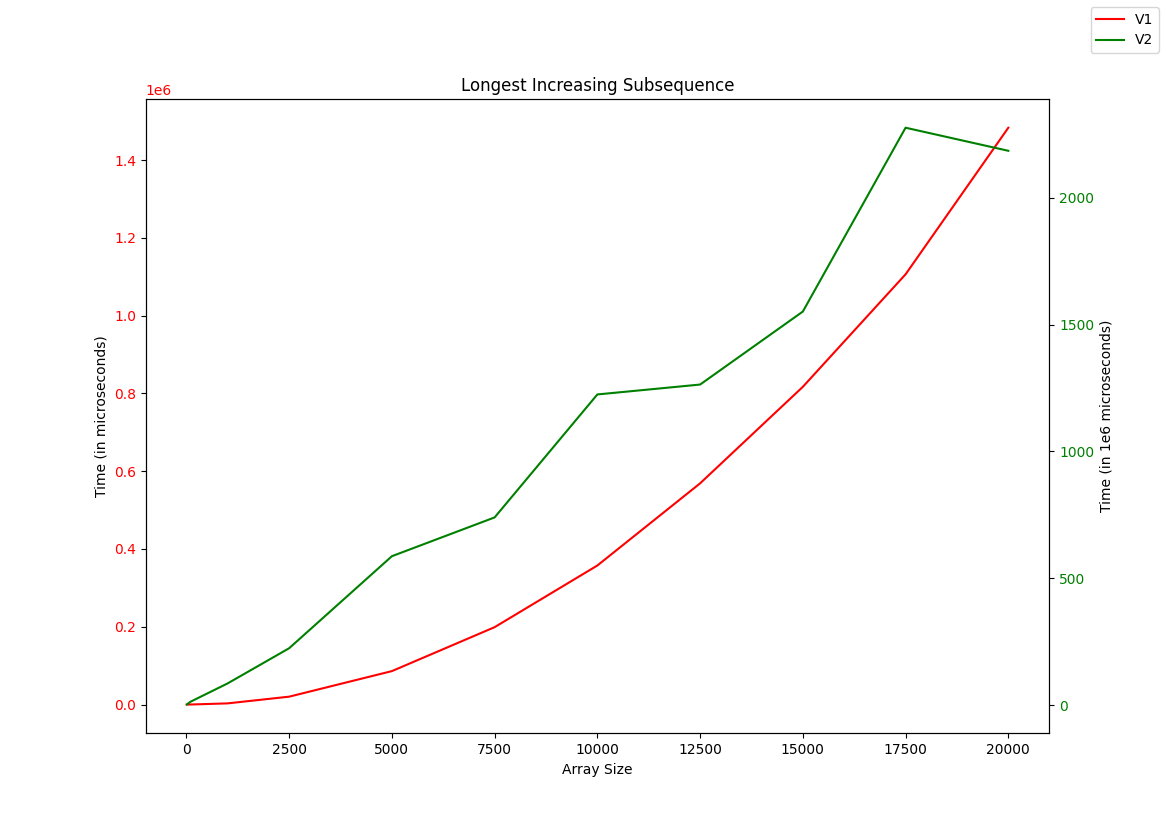
\includegraphics[scale=0.52]{img/LIS - multiple n values.png
    }
    \label{fig:LIS2}
    \caption{LIS: time taken, for different values of $n$}
\end{figure}

\section{Minimum Coins}

\subsection{Without Memoisation}
\begin{lstlisting}[language=C++]
int MinCoins::WithoutMemoisation(int n, const std::vector<int>& denom) {
    if (n == 0) return 0;
    int min = INT_MAX;
    for (auto& denomination : denom) {
        if (n - denomination >= 0) {
            min = std::min(min, 1 + WithoutMemoisation(n - denomination, denom));
        }
    }
    return min;
}
\end{lstlisting}

\subsection{With Memoisation}

\begin{lstlisting}[language=C++]
int MinCoins::WithMemoisationHelper(int n, const std::vector<int>& denom, std::vector<int>& CoinMemo) {
    if (CoinMemo[n] != -1) return CoinMemo[n];
    int min = INT_MAX;
    for (auto& denomination : denom) {
        if (n - denomination >= 0) {
            min = std::min(min, 1 + WithMemoisationHelper(n - denomination, denom, CoinMemo));
        }
    }
    CoinMemo[n] = min;
    return min;
}

int MinCoins::WithMemoisation(int n, const std::vector<int>& denom) {
    std::vector<int> CoinMemo(n + 1, -1);
    CoinMemo[0] = 0;
    return WithMemoisationHelper(n, denom, CoinMemo);
}
\end{lstlisting}

\begin{figure}[!h]
    \centering
    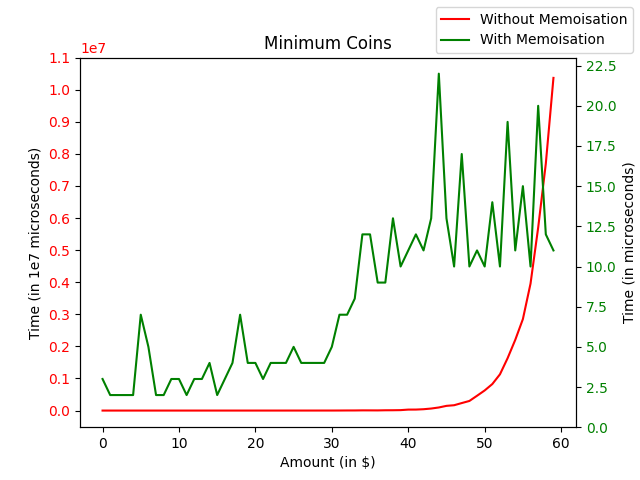
\includegraphics[scale=0.95]{img/Minimum Coins - Memo vs No Memo Graph.png}
    \label{fig:mincoins}
    \caption{Time taken to calculate the minimum number of coins needed with and without memoisation for the denominations 1, 5, 9 and 23}
\end{figure}

\section{0-1 Knapsack}
\begin{tcolorbox}
    \textbf{The Problem:} Given a knapsack with a maximum weight capacity $W$ and a set of $N$ items, each with its own weight $w$ and value $v$, find the maximum value of the items that can be fit into the knapsack. Each item must either be chosen or not chosen, hence this problem is called 0-1 knapsack problem.
\end{tcolorbox}

\subsection{A Greedy Approach}
One of the first few approaches that one might try to solve the 0-1 Knapsack problem is the greedy approach\textemdash to sort the items in decreasing order of $\frac{value}{weight}$ and choose items with the highest $\frac{value}{weight}$ ratios. However, this approach is incorrect. Consider the following counterexample.

\begin{center}
    $W = 10,\, N = 3$ \par
    \begin{tabular}{c | c | c | c}
        \hline
        S. No.        & 0   & 1   & 2     \\
        \hline
        $w$           & 5   & 5   & 8     \\
        $v$           & 4   & 4   & 7     \\
        $\frac{v}{w}$ & 0.8 & 0.8 & 0.875
    \end{tabular}
\end{center}
Using the greedy method, we would pick only item 2, as it has the highest $\frac{v}{w}$ ratio and might seem like the most efficient use of the available space at first glance. However, picking items 1 and 2 instead would give us a total value of 8, which is higher. Hence, the greedy approach is faulty.

\subsubsection{An Offshoot: Fractional Knapsack}
In this version of the problem, we are allowed to take fractional quantities of each item. That is, if one of the items was a kilogram of rice, then we'd be allowed to take anywhere from no rice to a few grams to the entire kilogram.

The greedy approach is a valid solution for the fractional knapsack problem. As the issue of space efficiency does not crop up anymore\textemdash since fractional items are allowed, the most efficient way to pack the knapsack will always be to fill it with items in descending order of $v/w$.

\subsection{0-1 Knapsack: With Repetition}
In this version of the problem, we are allowed to pick any number of each item. Let us create an array called `m' defined as
\begin{equation}
    m_w = \text{highest value possible with a knapsack of capacity } w.
\end{equation}
For each item $i$ and a knapsack of capacity $w$, we have two possibilities: either the optimal solution corresponding to $m_w$ contains item $i$ or it doesn't.
If the optimal solution corresponding to $m_w$ contains item $i$, then if we remove item $i$ from this set of items, we are left with the optimal solution to a knapsack with capacity $w - w_i$. This implies that $m_w$ is the maximum of at most $N$ possibilities\textemdash one for including / excluding each of the $N$ items in the optimal solution. Thus, the time complexity is $O(NW)$.

\begin{lstlisting}[language=C++]
int WithRepetition(int N, int W, const std::vector<int>& w, const std::vector<int>& v) {
    std::vector<int> m(N, 0);
    m[0] = 0;
    for (int capacity = 1; capacity <= W; ++capacity) {
        for (int i = 0; i < w.size(); ++i) {
            if (w[i] <= capacity) {
                m[capacity] = std::max(m[capacity], m[capacity - w[i] + v[i]]);
            }
        }
    }
}
\end{lstlisting}

\subsection{0-1 Knapsack: Without Repetition}
In this version of the problem, we are only allowed to pick one of each item.

Let us define $m(i, w)$ to be the maximum value that can be attained with the first $i$ items and a knapsack with capacity $w$. We need to find $m(N, W)$.
\begin{itemize}
    \item $m(0, w) = 0 \quad \forall w$ where $0 \leq w \leq W$.
    \item $m(i, 0) = 0 \quad \forall i$ where $0 \leq i < N$ (assuming zero-based indexing).
    \item $m(i, w) = m(i - 1, w)$ \quad if $w_i > w$ (that is, it's not possible to fit in the $i$th item)
    \item If $w_i \leq w$, there there are 2 possibilities. Either an optimal solution contains the $i$th item or it doesn't. If it doesn't, then $m(i, w) = m(i-1, w)$. If it does, $m(i, w) = m(i - 1, w - w_i) + v_i$. To find out which of these possibilities is optimal, we simply take their maximum.
          $$
              m(i, w) = \max \{ m(i-1, w), m(i-1, w-w_i) + v_i \}
          $$
\end{itemize}

The C++ program of the above algorithm is as follows.

\begin{lstlisting}[language=C++]
int KnapsackWithoutRepetition(int N, int W, const std::vector<int>& w, const std::vector<int>& v) {
  std::vector<std::vector<int>> m(N + 1, std::vector<int>(W + 1));
  for (int i = 0; i <= N; ++i) {
    for (int j = 0; j <= W; ++j) {
      if (i == 0 || j == 0)
        m[i][j] = 0;
      else if (j >= w[i-1])
        m[i][j] = std::max(m[i-1][j-w[i-1]] + v[i-1], m[i-1][j]);
      else 
        m[i][j] = m[i-1][j];
    }
  }
  return m[N][W];
}
\end{lstlisting}

\section{Longest Common Subsequence (LCS)} \label{LCS}
\begin{tcolorbox}
    \textbf{The Problem:} Given two sequences, find the longest sequence that is a subsequence of both of these sequences.
\end{tcolorbox}

We divide the LCS problem into subproblems that are simpler. That is, LCS has the optimal substructure property.

\begin{definition}[Prefix]
    The prefix $s_n$ of a string $s$ is defined as the first $n$ characters of $s$.
\end{definition}

\subsection{First Observation}
For any character \textit{A},
\begin{equation*}
    \textit{LCS(X+A, Y+A)} = \textit{LCS(X, Y)+A},
\end{equation*}
where + denotes concatenation.
% 
For example, \textit{LCS(`window', `widow') = LCS('windo', `wido') + `w'}.

\subsection{Second Observation}
If \textit{A} and \textit{B} are different characters, then \textit{LCS(X+A, Y+B)} is maximal-length string of the set \{\textit{LCS(X+A, Y), LCS(X, Y+B)}\}. If both have the same length, then any one of the two may be chosen.

\subsection{Algorithm}
From the two observations above, we come to the conclusion below.
\begin{equation}
    \textit{LCS(X\textsb{i}, Y\textsb{i})} = \begin{cases}
        \phi                                                                                                             & \text{if } i = 0 \text{ or } j = 0                         \\
        \textit{LCS(X\textsb{i-1}, Y\textsb{j-1})+x\textsb{i}}                                                           & \text{if } i, j > 0 \text{ and } x\textsb{i} = y\textsb{j} \\
        \text{maximal length of } \{\textit{LCS(X\textsb{i-1}, Y\textsb{j})}, \textit{LCS(X\textsb{i}, Y\textsb{j-1})}\} & \text{Otherwise}                                           \\
    \end{cases}
\end{equation}
Initially, \textit{i} and \textit{j} are the lengths of the strings \textit{X} and \textit{Y} respectively.

A similar algorithm could also be written using suffixes.

\subsection{Time Complexity}
For only two sequences, the time complexity is at worst quadratic in the length of the longer sequence (when no pair of characters of the two seqeunces matches) and at best linear (when the two sequences are identical). Mathematically,
\begin{gather*}
    T(n) = O(n^2),\text{ and} \\
    T(n) = \Omega(n)
\end{gather*}
where $n$ is the length of the longer sequence of the two given ones.

In general, in order to find the LCS of $k$ sequences, the problem becomes NP-hard and the time complexity becomes $O(n^k)$, where $n$ is the length of the longest sequence of the $k$ given sequences.

\subsection{C++ Implementation}
\begin{lstlisting}[language=C++]
#include <iostream>
#include <string>

std::string LCS(const std::string& a, const std::string& b, int i, int j) {
    if (i == -1 || j == -1)
        return "";
    else if (i == j) {
        return LCS(a, b, i - 1, j - 1) + a[i];
    } else {
        std::string x = LCS(a, b, i - 1, j);
        std::string y = LCS(a, b, i, j - 1);
        return x.size() > y.size() ? x : y;
    }
}

int main(void) {
    std::string a, b;
    std::cin >> a >> b;

    std::cout << "LCS: " << LCS(a, b, a.size(), b.size());

    return 0;
}
\end{lstlisting}

\section{Shortest Common Supersequence (SCS)}
\begin{definition}
    $X$ is said to be a supersequence of $Y$ if $Y$ is a subsequence of $X$.
\end{definition}

\begin{tcolorbox}
    \textbf{The Problem:} Given two seqeuces, find the shortest sequence that is a supersequence of both of these sequences.
\end{tcolorbox}

For example, for the strings `window' and `widow', the SCS is `window'. For `mouse' and `blouse', there are multiple possible shortest common supersequences, of which we can choose any. They are `mblouse', `bmlouse' and `blmouse'.

\subsection{Algorithm}
Let $X$ and $Y$ be the two sequences whose SCS we wish to find.
\begin{enumerate}
    \item Find the longest common subsequence of $X$ and $Y$. (Refer to \cref{LCS}.)
    \item Insert the characters in $X$ and $Y$ that are not in their LCS into the LCS, while maintaining their relative order to the LCS characters.
\end{enumerate}

For example, let $X=$ `overlap' and $Y=$ `rapper'. Their LCS is `rap'. Now, we insert the non-LCS characters in $X$ (namely `ovel') and $Y$ (namely `per') into `rap'. The SCS becomes `overlapper'. There is only one SCS in this case.

Now consider $X=$ `subsequence' and $Y=$ `supersequence'. Their LCS is `susequence'. The non-LCS characters in $X$ are `b' and in $Y$ are `per'.
All possible shortest common supersequences are `subpersequence', `supbersequence', `supebrsequence', and `superbsequence'.

\subsection{Time Complexity}
The time complexity is identical to that of the LCS problem. For $k$ input sequences of maximum length $n$, the time complexity is $O(n^k)$.

\section{Tower of Hanoi}
This is one of my all-time favourite problems and a classic puzzle that was coined by French mathematician Édouard Lucas in 1883. The problem, while easy to understand, might have one scratching their heads for days or weeks.

\begin{tcolorbox}
    \textbf{The Problem:} There are 3 rods (let's call then rods 1, 2 and 3) and $n$ discs with holes in their centres that would fit a rod. No two discs are of the same size. All of the discs are initially on rod 1, such that the largest disc is at the bottom and every other disc is on top of a larger disc. Each move in the game consists of removing the topmost disc in a rod and placing it on top of another rod's stack, subject to the rule that a rod may only be placed on top of a larger rod.

    What is the minimum number of moves needed to move all the discs from rod 1 to rod 3 and what are they?
\end{tcolorbox}

\begin{figure}[!h]
    \centering
    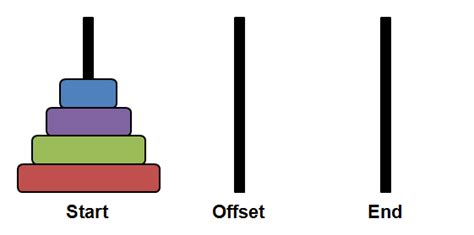
\includegraphics[scale=1]{img/Tower of Hanoi - Sample.png}
\end{figure}

I recommend trying out a few examples for yourself before looking at the solution. Mathsiffun.com has a nice webpage for to play the puzzle \href{https://www.mathsisfun.com/games/towerofhanoi.html}{here}.

\subsection{Examples}
For $n=1$, trivially, we just move the disc from rod 1 to rod 3.

For $n=2$, move the topmost disc to rod 2, then move the disc in rod 1 to rod 3 and finally put the other disc on rod 2 in rod 3.

Observe that all we need to describe a move is the source and destination rod that was used to move the disc in that move. Thus, for the sake of brevity, we shall use this to denote the moves for $n=3$:
\begin{enumerate}[noitemsep]
    \item rod 1 $\rightarrow$ rod 3
    \item rod 1 $\rightarrow$ rod 2
    \item rod 3 $\rightarrow$ rod 2
    \item rod 1 $\rightarrow$ rod 3
    \item rod 2 $\rightarrow$ rod 1
    \item rod 2 $\rightarrow$ rod 3
    \item rod 1 $\rightarrow$ rod 3
\end{enumerate}

\subsection{Minimum Number of Moves Needed}
By taking a few examples and looking for a pattern, we might come to the conclusion that the minimum number of moves needed for the puzzle with $n$ discs is $2^n - 1$. In fact, this is true. Let's prove this using mathematical induction.
\begin{proof}
    We need to prove two claims:
    \begin{enumerate}
        \item It is always possible to solve the puzzle in $2^n-1$ moves.
        \item It is impossible to solve it in less than $2^n-1$ moves.
    \end{enumerate}

    Let us first prove the first claim. The induction hypothesis is that it is always possible to solve the puzzle in $2^n-1$ moves.
    \begin{description}
        \item[Base case.] For $n=1$, we need only one move. This is trivially shown to be true.
        \item[Induction step.] From the induction hypothesis, we assume that we can move $n$ discs from rod 1 to rod 3 in $2^n - 1$ moves. We need to show that assuming this to be true, the hypothesis holds also true for $n+1$ discs. This is elegantly shown. To move $n+1$ discs from rod 1 to rod 3, we
            \begin{itemize}
                \item first move the topmost $n$ discs to rod 2 in $2^n-1$ moves,
                \item then move the bottom-most disc from rod 1 to rod 3 in 1 move, and,
                \item then move the $n$ discs from rod 2 to rod 3 in $2^n-1$ moves.
            \end{itemize}
            The total number of moves used is $(2^n - 1) + 1 + (2^n - 1) = 2 * 2^n - 1 = 2^{n+1} - 1$.
            Thus, the induction hypothesis holds true and it is always possible to solve a Tower of Hanoi puzzle with $n$ discs in $2^n-1$ moves.
    \end{description}

    Now, we shall prove that $2^n - 1$ is indeed the minimum possible number of moves need to solve it (this is the induction hypothesis).
    \begin{description}
        \item[Base case.] For $n=1$, trivially, the number of moves needed is 1, which is equal to $2^1 - 1$.
        \item[Induction step.] Now consider the induction hypothesis for $n+1$ discs. Observe that in order to move a disc from rod 1 to rod 3, all other discs smaller than this disc \textit{must} be on rod 2. So, in order to move $n+1$ discs from rod 1 to rod 3, it is imperative to move the top $n$ discs to rod 2 first, then move the largest disc to rod 3, and then move the $n$ discs from rod 2 to rod 3. From the induction hypothesis, this takes a minimum of $2^n-1$ moves, 1 move, and $2^n - 1$ moves. Summing them up, we get $2^{n+1}-1$ moves. Thus, from the principle of mathematical induction, the minimum number of moves needed to solve the Tower of Hanoi puzzle with $n$ discs is $2^n - 1$ moves.
    \end{description}
\end{proof}

\subsection{Algorithm}
The recursive algorithm, as already mentioned above, is simply to move $n-1$ discs from rod 1 to rod 2, then move 1 disc from rod 1 to rod 3, and finally move $n-1$ discs from rod 2 to rod 2. The recursion stops when there's only 1 disc in a rod, in which case we simply move it to its destination without any recursion. We store the moves we made in an array called `\texttt{Moves}'. Each move can be uniquely characterised by the source rod and the destination rod (along with the index in \texttt{Moves}, but that is not something we need to store explicitly), so that is what we shall store for each move.

\begin{lstlisting}[language=C++]
// Move n discs from source to dest, assuming that it is possible
// to do so without moving the discs on the 2 rods other than the  source rod.
// `Moves' is a list of pairs - Move[i] stores the source and the
// destination rod for the ith move
void MoveDisc(int n, int source, int dest, std::vector<std::pair<int, int>>& Moves) {
    if (n == 1) {
        Moves.push_back({source, dest});
        return;
    }
    int otherRod = 6 - source - dest;  // whichever of {1,2,3} is not source or dest
    MoveDisc(n - 1, source, otherRod, Moves);
    Moves.push_back({source, dest});
    MoveDisc(n - 1, otherRod, dest, Moves);
}
\end{lstlisting}

\section{Bellman-Ford Algorithm}
\begin{tcolorbox}
    \textbf{The Problem:} Given a weighted graph $G=(V,E)$ and a vertex $s$, find the shortest distance from $s$ to all the vertices in $V$.
\end{tcolorbox}

The Bellman-Ford algorithm is used to find the single-source shortest path in both directed and undirected graphs and even in unweighted graphs. It is often used in real life in many protocols in the internet such as the routing information protocol and the distance-vector routing protocol, usually for transmitting information on a network.

Notice that if the graph contains negative edge cycles, then that implies that for some vertices, the shortest distance does not exist, i.e. it is $-\infty$.

We use the idea of relaxation in the Bellman-Ford algorithm. Relaxation refers to gradually and continuously shortening the distance between vertices.
Let $E = \{e_1, e_2, \ldots, e_{|E|}\}$ and $V = \{v_1, v_2,\ldots, v_{|V|}\}$. Let $w_{e_i}$ refer to the weight of $e_i$.
Then the algorithm is as follows:
\begin{enumerate}
    \item Initialiase the distance from $s$ to every vertex as infinity.
    \item For every vertex, create a `previous' vertex which is the vertex that appears before it in the shortest path to $s$. Initially, this is unknown.
    \item Set the distance from $s$ to itself as 0.
    \item Then, $|V|-1$ times, iterate over every edge in $E$ and relax it.
    \item Relaxation of an edge $e = (u, v)$ is the process of checking if the previously known shortest distance from $s$ to $v$ is longer than the path from $s$ to $u$ to $v$, and if it is, setting the new shortest distance to $v$ as the distance from $s$ to $u$ + $w_{(u, v)}$.
\end{enumerate}

\subsection{Pseudocode}
\begin{lstlisting}[mathescape=true]
for v in V:
    dist[v] = infinity
    prev[v] = None
dist[s] = 0
for i in [1 ... |V|-1]:
    for (u, v) in E:
        relax(u, v)

function relax(u, v):
    if dist[v] > dist[u] + w$_{\texttt{(u, v)}}$:
        dist[v] = dist[u] + w$_{\texttt{(u, v)}}$
        prev[v] = u
\end{lstlisting}

\subsection{Time Complexity}
Dijkstra's algorithm is faster than the Bellman-Ford algorithm at $O(V + E)$, but the latter can handle negative edge weights which the former cannot.

Each relaxation operation takes $O(1)$ and we perform $(|V|-1)\cdot|E|$ iterations. Therefore, the worst-case time complexity is $O(|V|\cdot|E|)$.



\section{Floyd-Warshall Algorithm}
\begin{tcolorbox}
    \textbf{The Problem:} Find the shortest path between all pairs of vertices in a graph with weighted edges assuming that the graph contains no negative cycle (i.e., cycles whose sum of edge weights is negative).
\end{tcolorbox}

Let the given graph be $G = (V, E)$ where $V$ is the set of vertices and $E$ is the set of weighted edges.
Then, the Floyd-Warshall algorithm is as follows.
\begin{enumerate}
    \item Initialise the shortest path between every pair of vertices to infinity.
    \item Define an array called `\texttt{dist}' as follows.
          \begin{equation}
              \texttt{dist[i][j]} = \text{shortest path from vertex \texttt{i} to vertex \texttt{j}}.
          \end{equation}
    \item Find the shortest path between every pair of vertices that used 0 intermediate vertices (i.e., there were 0 vertices between the source and destination vertices). Then, do the same for 1 intermediate vertex, 2 intermediate vertices, and so on till $|V|$ intermediate vertices.
    \item Throughout step 2, keep track of the minimum distance between every pair of vertices over every possible number of intermediate vertices in \texttt{dist}.
\end{enumerate}

\subsection{Pseudocode} \label{floydwarshall:pseudocode}
\begin{lstlisting}
Create a |V| x |V| matrix, dist, that will describe the distances between vertices
for each cell (i, j) in dist:
    if i == j:
        dist[i][j] = 0
    if (i, j) is an edge in E:
        dist[i][j] = weight(i, j)       ## Given as input
    else:
        dist[i][j] = infinity
for k from 1 to |V|:
    for i from 1 to |V|:
        for j from 1 to |V|:
            if dist[i][j] > dist[i][k] + dist[k][j]:
                dist[i][j] = dist[i][k] + dist[k][j]
\end{lstlisting}

\subsection{C++ Implementation}
\begin{lstlisting}[language=C++]
#include <iostream>

void FloydWarshall(int **dist, int v) {
    for (int k = 0; k < v; ++k) {
        for (int i = 0; i < v; ++i)
            for (int j = 0; j < v; ++j)
                if (dist[i][k] + dist[k][j] < dist[i][j]) {
                    dist[i][j] = dist[i][k] + dist[k][j];
                }
    }
}

int main(void) {
    int v, e;
    std::cout << "Enter number of vertices: ";
    std::cin >> v;

    std::cout << "Enter number of edges: ";
    std::cin >> e;

    int **dist = new int *[v];
    for (int i = 0; i < v; ++i) {
        dist[i] = new int[v];
        for (int j = 0; j < v; ++j) {
            if (i == j)
                dist[i][j] = 0;
            else
                dist[i][j] = INT_MAX;
        }
    }

    std::cout << "Enter the edges in this format: `tail head weight'"
                << "\n";
    for (int a = 0; a < e; ++a) {
        int i, j, w;
        std::cin >> i >> j >> w;
        dist[i][j] = w;
    }

    FloydWarshall(dist, v);

    std::cout << "The minimum distance matrix is:\n";
    for (int i = 0; i < v; ++i) {
        for (int j = 0; j < v; ++j) {
            std::cout << dist[i][j] << " ";
        }
        std::cout << "\n";
    }

    for (int i = 0; i < v; ++i) {
        delete[] dist[i];
    }
    delete[] dist;
    return 0;
}
\end{lstlisting}

\subsection{Time Complexity}
From lines 9 to 12 of the pseudocde (see \cref{floydwarshall:pseudocode}), it is clear that the algorithm contains three nested loops, each with $|V|$ iterations. Thus, the time complexity is $O(|V|^3)$.

\end{document}